
\begin{figure}[t]
\centering
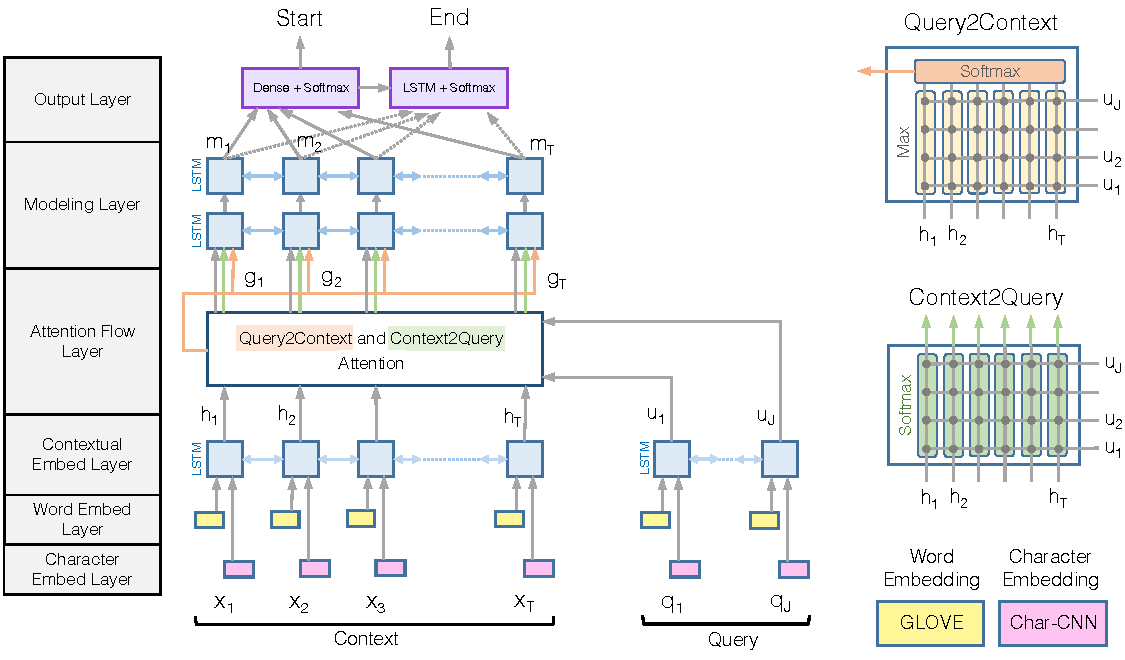
\includegraphics[width=34pc]{figures/model}
\caption{\small BiDirectional Attention Flow Model\space\space \textit{(best viewed in color)}}
\label{fig:model}
\end{figure}
Our machine comprehension model is a hierarchical multi-stage process and consists of six layers (Figure~\ref{fig:model}): 
\begin{enumerate}
    \item \textbf{Character Embedding Layer} maps each word to a vector space using character-level CNNs. %(Section~\ref{subsec:char})
    \item \textbf{Word Embedding Layer} maps each word to a vector space using a pre-trained word embedding model. %(Section~\ref{subsec:emb})
    \item \textbf{Contextual Embedding Layer} utilizes contextual cues from surrounding words to refine the embedding of the words. %(Section~\ref{subsec:pre})\\
    These first three layers are applied to both the query and context.
    \item \textbf{Attention Flow Layer} %(Section~\ref{subsec:att})
    couples the query and context vectors and produces a set of query-aware feature vectors for each word in the context.
    \item \textbf{Modeling Layer} employs a Recurrent Neural Network to scan the context.% (Section~\ref{subsec:main})
    \item \textbf{Output Layer} provides an answer to the query.% (Section~\ref{subsec:out})
\end{enumerate}

\paragraph{1. Character Embedding Layer.}\label{subsec:char}
Character embedding layer is responsible for mapping each word to a high-dimensional vector space. Let $\{\bm{x}_1, \dots \bm{x}_T\}$ and $\{\bm{q}_1, \dots \bm{q}_J\}$ represent the words in the input context paragraph and query, respectively.
Following~\cite{char-cnn}, we obtain the character-level embedding of each word using Convolutional Neural Networks (CNN). Characters are embedded into vectors, which can be considered as 1D inputs to the CNN, and whose size is the input channel size of the CNN. The outputs of the CNN are max-pooled over the entire width to obtain a fixed-size vector for each word.  

\paragraph{2. Word Embedding Layer.}\label{subsec:emb}
Word embedding layer also maps each word to a high-dimensional vector space. We use pre-trained word vectors, GloVe~\citep{glove}, to obtain the fixed word embedding of each word.

The concatenation of the character and word embedding vectors is passed to a two-layer Highway Network~\citep{highway}. 
The outputs of the Highway Network are two sequences of $d$-dimensional vectors, or more conveniently, two matrices: ${\bf X} \in \mathbb{R}^{d \times T}$ for the context and ${\bf Q} \in \mathbb{R}^{d \times J}$ for the query.

\paragraph{3. Contextual Embedding Layer.}\label{subsec:pre}
We use a Long Short-Term Memory Network (LSTM)~\citep{lstm} on top of the embeddings provided by the previous layers to model the temporal interactions between words. %In particular, we use a Long Short-Term Memory Network (LSTM)~\citep{lstm}, a popular subclass of RNNs with memory channel and gating mechanism.
We place an LSTM in both directions, and concatenate the outputs of the two LSTMs. Hence we obtain ${\bf H} \in \mathbb{R}^{2d \times T}$ from the context word vectors ${\bf X}$, and ${\bf U} \in \mathbb{R}^{2d \times J}$ from query word vectors ${\bf Q}$.
Note that each column vector of ${\bf H}$ and ${\bf U}$ is $2d$-dimensional because of the concatenation of the outputs of the forward and backward LSTMs, each with $d$-dimensional output.

It is worth noting that the first three layers of the model are computing features from the query and context at different levels of granularity, akin to the multi-stage feature computation of convolutional neural networks in the computer vision field.

\paragraph{4. Attention Flow Layer.}\label{subsec:att}
Attention flow layer is responsible for linking and fusing information from the context and the query words. 
Unlike previously popular attention mechanisms~\citep{memnn,hill2015goldilocks,iterative,reasonet}, the attention flow layer is not used to summarize the query and context into single feature vectors. 
Instead, the attention vector at each time step, along with the embeddings from previous layers, are allowed to flow through to the subsequent modeling layer. 
This reduces the information loss caused by early summarization.
 
The inputs to the layer are contextual vector representations of the context ${\bf H}$ and the query ${\bf U}$. 
The outputs of the layer are the query-aware vector representations of the context words, ${\bf G}$, along with the contextual embeddings from the previous layer.

In this layer, we compute attentions in two directions: from context to query as well as from query to context. 
Both of these attentions, which will be discussed below, are derived from a shared similarity matrix, ${\bf S} \in \mathbb{R}^{T \times J}$, between the contextual embeddings of the context (${\bf H}$) and the query (${\bf U}$), 
where ${\bf S}_{tj}$ indicates the similarity between $t$-th context word and $j$-th query word.
The similarity matrix is computed by
\begin{equation}\label{eqn:sim}
{\bf S}_{tj} = \alpha({\bf H}_{:t}, {\bf U}_{:j}) \in \mathbb{R}
\end{equation}
where $\alpha$ is a trainable scalar function that encodes the similarity between its two input vectors,
${\bf H}_{:t}$ is $t$-th column vector of ${\bf H}$, and
${\bf U}_{:j}$ is $j$-th column vector of ${\bf U}$,
We choose $\alpha({\bf h}, {\bf u}) = {\bf w}^\top_{({\bf S})} [{\bf h}; {\bf u}; {\bf h} \circ {\bf u}]$,
where ${\bf w}_{({\bf S})} \in \mathbb{R}^{6d}$ is a trainable weight vector, 
$\circ$ is elementwise multiplication,
$[;]$ is vector concatenation across row,
and implicit multiplication is matrix multiplication.
Now we use ${\bf S}$ to obtain the attentions and the attended vectors in both directions.

%\vspace{.1cm}
\textbf{\ \ \ Context-to-query Attention.} 
Context-to-query (C2Q) attention signifies which query words are most relevant to each context word.
Let ${\bf a}_t \in \mathbb{R}^J$ represent the attention weights on the query words by $t$-th context word, $\sum {\bf a}_{tj} = 1$ for all $t$. The attention weight is computed by ${\bf a}_t = \mathrm{softmax}({\bf S}_{t:}) \in \mathbb{R}^J$,
and subsequently each attended query vector is $\tilde{{\bf U}}_{:t} = \sum_j {\bf a}_{tj} {\bf U}_{:j}$.
Hence $\tilde{{\bf U}}$ is a $2d$-by-$T$ matrix containing the attended query vectors for the entire context.

\textbf{\ \ \ Query-to-context Attention.}
Query-to-context (Q2C) attention signifies which context words have the closest similarity to one of the query words and are hence critical for answering the query. We obtain the attention weights on the context words by ${\bf b} = \mathrm{softmax}(\max_{col} ({\bf S})) \in \mathbb{R}^T$, where the maximum function ($\max_{col}$) is performed across the column. Then the attended context vector is $\tilde{\bf h} = \sum_t {\bf b}_t {\bf H}_{:t} \in \mathbb{R}^{2d}$. This vector  indicates the weighted sum of the most important words in the context with respect to the query.
$\tilde{\bf h}$ is tiled $T$ times across the column, thus giving $\tilde{\bf H} \in \mathbb{R}^{2d \times T}$.

Finally, the contextual embeddings and the attention vectors are combined together to yield ${\bf G}$, where each column vector can be considered as the query-aware representation of each context word.
We define ${\bf G}$ by
\begin{equation}\label{eqn:flow}
{\bf G}_{:t} = {\bm \beta}({\bf H}_{:t}, \tilde{\bf U}_{:t}, \tilde{\bf H}_{:t}) \in \mathbb{R}^{d_{\bf G}}
\end{equation}
where ${\bf G}_{:t}$ is the $t$-th column vector (corresponding to $t$-th context word),
${\bm \beta}$ is a trainable vector function that fuses its (three) input vectors,
and $d_{\bf G}$ is the output dimension of the ${\bm \beta}$ function.
While the ${\bm \beta}$ function can be an arbitrary trainable neural network, such as multi-layer perceptron, 
a simple concatenation as following still shows good performance in our experiments: ${\bm \beta}({\bf h}, \tilde{\bf u}, \tilde{\bf h}) = [{\bf h}; \tilde{\bf u}; {\bf h} \circ \tilde{\bf u}; {\bf h} \circ \tilde{\bf h}] \in \mathbb{R}^{8d \times T}$ (i.e., $d_{\bf G} = 8d$).

\paragraph{5. Modeling Layer.}\label{subsec:main}
The input to the modeling layer is  ${\bf G}$, which encodes the query-aware representations of context words.
The output of the modeling layer captures the interaction among the context words conditioned on the query.
This is different from the contextual embedding layer, which captures the interaction among context words independent of the query. 
We use two layers of bi-directional LSTM, with the output size of $d$ for each direction. 
Hence we obtain a matrix ${\bf M}\in \mathbb{R}^{2d \times T}$, which is passed onto the output layer to predict the answer. 
Each column vector of ${\bf M}$ is expected to contain contextual information about the word with respect to the entire context paragraph and the query.

\paragraph{6. Output Layer.}\label{subsec:out}
The output layer is application-specific. 
The modular nature of \sysshort\ allows us to easily swap out the output layer based on the task, with the rest of the architecture remaining exactly the same. Here, we describe the output layer for the QA task. In section~\ref{subsec:cnn-details}, we use a slight modification of this output layer for cloze-style comprehension.  %the design of the layer when the answer lies within the context paragraph; that is, the answer is a contiguous subset of the context paragraph words.

The QA task requires the model to find a sub-phrase of the paragraph to answer the query. The phrase is derived by predicting the start and the end indices of the phrase in the paragraph. We obtain the probability distribution of the start index over the entire paragraph by
\begin{equation}
{\bf p}^{1} = \mathrm{softmax}({\bf w}_{({\bf p}^1)}^\top[{\bf G};{\bf M}]),
\end{equation}
where ${\bf w}_{({\bf p}^1)} \in \mathbb{R}^{10d}$ is a trainable weight vector.
For the end index of the answer phrase, we pass ${\bf M}$ to another bidirectional LSTM layer and obtain ${\bf M}^2 \in \mathbb{R}^{2d \times T}$.
Then we use ${\bf M}^2$ to obtain the probability distribution of the end index in a similar manner:
\begin{equation}
{\bf p}^{2} = \mathrm{softmax}({\bf w}_{({\bf p}^2)}^\top[{\bf G};{\bf M}^2])
\end{equation}

\textbf{Training.}
We define the training loss (to be minimized) as the sum of the negative log probabilities of the true start and end indices by the predicted distributions, averaged over all examples:
\begin{equation}
L(\theta) = -\frac{1}{N}\sum^N_i \log({\bf p}^1_{y^1_i}) + \log({\bf p}^2_{y^2_i})
\end{equation}
where $\theta$ is the set of all trainable weights in the model (the weights and biases of CNN filters and LSTM cells, ${\bf w}_{({\bf S})}$, ${\bf w}_{({\bf p}^1)}$ and ${\bf w}_{({\bf p}^2)}$),
$N$ is the number of examples in the dataset,
$y^1_i$ and $y^2_i$ are the true start and end indices of the $i$-th example, respectively,
and ${\bf p}_k$ indicates the $k$-th value of the vector ${\bf p}$.

\textbf{Test.}
The answer span $(k, l)$ where $k \leq l$ with the maximum value of ${\bf p}^1_k {\bf p}^2_l$ is chosen, which can be computed in linear time with dynamic programming.